\documentclass[12pt]{article}
% This work is about rootkits
\usepackage[T2A]{fontenc}
\usepackage[utf8]{inputenc}
\usepackage{multicol}
\usepackage{gensymb}
\usepackage{graphicx}
\usepackage{listings}
\usepackage{verbatim}

\usepackage{hyperref}
\hypersetup{colorlinks, 
           citecolor=black,
           filecolor=black,
           linkcolor=black,
           urlcolor=black,
           bookmarksopen=true,
           pdftex}

\hfuzz = .6pt % avoid black boxes

\title{Kernel rootkits in Linux: low-level approach and prevention}
\date{}
\author{Ivan Galinskiy}

\begin{document}
\maketitle

\newpage
  \emph{
  Copyright (C) 2010 Ivan Galinskiy.
    Permission is granted to copy, distribute and/or modify this document
    under the terms of the GNU Free Documentation License, Version 1.3
    or any later version published by the Free Software Foundation;
    with no Invariant Sections, no Front-Cover Texts, and no Back-Cover Texts.
    A copy of the license is included in the section entitled "GNU
    Free Documentation License".}
  \newpage
  
  \section{Kinds of rootkits}
  \subsection{Classification}
  What exactly are the rootkits? In the malware classification, rootkits are
  programs designed to hide the fact of system intrusion by hiding processes,
  users, files etc. This is the base classification, which is true for all
  kinds of rootkits. But if we look at real samples, deviations appear. For
  example, in some cases the rootkit is not just ``standalone'', but a part of
  another piece of malware which is being hidden. A very good example is
  Rustock.C designed for Windows.

  \subsection{Basic principles of work}
  Obviously, the process of hiding something is based on modifying system
  ``internals'', requiring thus some way to gain administrative (root)
  privileges. This can be done in very different ways, and besides, it is not
  part of rootkit's job, so we will skip that. But there are basically two
  ways the rootkit ``holds'' itself on the main system:
  \begin{enumerate}
    \item Modifying files on the filesystem. When a program has administrative
      rights on the target machine, it can (almost always) do whatever it
      ``wants''. For example, modifying the passwd or sudo utilities will
      probably get users' passwords. The disadvantages are obvious. To detect
      the rootkit, the user needs to check main utilities' checksums from a
      trusted operating system (either by loading with LiveCD or by taking the
      harddisk to another machine).

    \item Modifying only the RAM. Of course, at first sight it may look a bit
      strange, as with a reboot anything will return to normal. But just
      imagine a server with, lets say, 2 years uptime? Now it looks better,
      and this kind of rootkits is much tougher (and more interesting to
      research).
  \end{enumerate}

  \section{A brief look at DR Linux rootkit}
  
  Well, finding this one was not a difficult task. Besides, it's one of the
  most up-to-date open-source rootkits available. Others are either very old,
  or don't match our context, so we will not look at them. The source code
  indicates that this rootkit is based on debug registers. According to Intel
  documentation, the debugging registers are DR0 - DR7. DR0 - DR3 registers
  hold four linear addresses. DR4 and DR5 are reserved for extended debugging
  and we are not going to look at them now. DR6 is the ``Debug State
  Register'' and DR7 is the ``Debug Control Register''. What is their purpose?
  The below scheme from Intel documentation explains some things.
  \begin{figure}[h]
    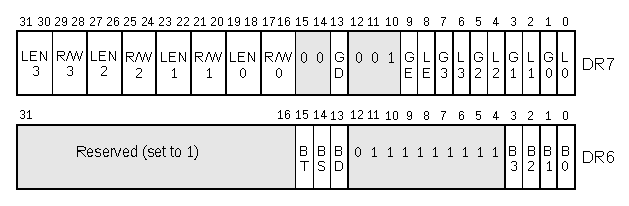
\includegraphics[width=\linewidth, keepaspectratio]{dregs}
  \end{figure}
  The one interesting is the DR7, which controls the debugging behaviour. For
  the rootkit, the usefullness is in the ability to control read, write or
  execute operations (or their combinations) on the breakpoints (note: the
  settings are individual for each breakpoint). Obviously, the breakpoints are
  not useful by themselves. When a breakpoint is reached, after executing it,
  the processor emits a \verb!#DB! exception, which is catched by the kernel
  handler in normal cases. But the rootkit changes the handler in Interrupt
  Descriptor Table to its own or either modifies the system handler (in this
  case the IDT remains untouched).

  \section{Interception techniques}

  Wait, is this the only way to control system internals? Actually, more
  methods were created through the time, but all of them are based on
  modifying well-known system structures, the quantity of which is not so
  big. What structures? Some of them are IDT, MSR, DR registers (as seen
  above), syscall tables... What are all these abbreviatures? They may look
  scary at first sight, but the things are simpler. So what all those things
  do?

  \begin{itemize}
    \item IDT means Interrupt Descriptor Table. In simple words, it contains
      addresses of handlers for interrupts. As we have seen in the DR rootkit,
      it may be very useful. There is also another detail, before Pentium II
      was introduced, system calls (i.e. calls from user applications to
      kernel) were performed using the \verb!0x80!  interrupt (loading the
      system call number into EAX register before invoking interrupt). And
      guess what? The pointer to the handler for that interrupt was stored in
      IDT too.

    \item MSR stands for Model Specific Registers. Before Pentium II,
      interrupts were used to make system calls. It's a simple way, but
      unfortunately, slow. That's why \verb!SYSENTER/SYSCALL! and
      \verb!SYSEXIT/SYSRET! (for Intel/AMD respectively) commands were
      introduced, providing a faster way to make system calls. Now the pointer
      to that handler of the call was not in IDT, but in a set of MSR
      registers. They store the target instruction, stack segment pointer
      etc. But the most interesting and useful for us is the
      \verb!IA_32_SYSENTER_EIP! which stores the target instruction. Changing
      it to something else will redirect all the system calls into the new
      procedure.

    \item So what is the difference between the above two methods? Only the
      way to \emph{call} system procedures! Even if we examine the source of
      \verb!system_call! and \verb!ia32_sysenter_target! (there is where
      \verb!IA_32_SYSENTER_EIP!  points by default), in both we find
      ``\verb!call *sys_call_table(,%eax,4)!''. This means that those
      procedures are the same in both cases (otherwise, it would be
      strange). And, of course, modifying pointers in this table can be very
      funny for the rootkit (and more for the machine owner).
  \end{itemize}


  \subsection{Modifying IDT}
  There are some other ways, of course, but now we will concentrate on the
  ones listed above and try to perform these ``tricks''. So, the first in the
  list is interception of interrupts via IDT. Ok, let's begin.
  \begin{itemize}
    \item First of all, I am going to be as kernel version independent as I
      can. It means that I am going to use resources available in the
      processor rather that predefined macros or whatever.
      
    \item OK, before we make any changes to IDT, we obviously need to know
      where exactly it resides. An assembly command \verb!SIDT! can help us
      with this, getting the IDTR register contents. In 32-bit systems, IDTR
      contains two fields: the 16-bit limit, specifying the size of the table,
      and 32-bit address which is the location of IDT. But there is a detail
      that led me to mistakes: the address is stored with low-order bytes
      first! We can define a function to get the register contents in
      easily-readable form: \verbatiminput{sidt.h}

    \item Half of the job is done now. However, we still need to get a
      particular entry in the IDT (to store the original interrupt handler,
      for example). In Linux on 32-bit systems, each entry in IDT is 8-bytes
      long and consists of an offset to the handler and some attributes. The
      funny thing is the offset is not continuous in the entry! The first 16
      bits begin at bit 0 of the IDT entry, and the last 16 are at the end of
      the entry. Tricky, right? The following code can handle with this:
      \verbatiminput{idt.h}

    \item Very good! Now that we have the entries, many things can be
      done. But let's stop with IDT hooking and continue to the next method.
  \end{itemize}

  \subsection{SYSENTER/SYSCALL interception}
  Well, this one is a juicy one! As I already told, beginning with Pentium II,
  Intel processors implemented the new \verb!SYSENTER!/\verb!SYSEXIT!
  instructions (and AMD used \verb!SYSCALL!/\verb!SYSRET!). They decreased the
  overhead of switching from user mode and vice-versa (the interrupts are
  slow). These instructions used special MSR registers to know where the
  target procedure was located. There is one that is specially relevant to us:
  \verb!SYSENTER_EIP_MSR!. Its contents are loaded to the EIP register
  (basically a jump) at the end of \verb!SYSENTER! execution. Initially it
  points to a kernel procedure, but we can change it to our procedure. How can
  it be done?
  \begin{itemize}
    \item First, of course, we need a way to access the
      \verb!SYSENTER_EIP_MSR! register. It's not accessed like the, let's say,
      EAX register. There is a special instruction, \verb!RDMSR!, that does
      it. The only requirement is that the number of MSR register should be
      loaded into ECX (the number of \verb!SYSENTER_EIP_MSR! is 0x176). The
      contents are stored in EDX and EAX registers (EDX is 0 on 32-bit
      systems).
      
    \item Now we can put a new value to the register. This process is
      basically an inverted version of the previous. We load the new value
      into EDX:EAX (EDX is zero, EAX is the new procedure pointer), the MSR
      register number into ECX, and perform the instruction \verb!WRMSR!.
  
    \item I thought that an example would be more helpful than a dry
      description, so here is a minimal sample kernel module for this task
      (the includes were (duh) excluded). It's a kernel module because
      \verb!WRMSR!  can only be performed at ring 0: \verbatiminput{msr.h}
      
    \item Obviously, this module doesn't do anything special, it's more like a
      ``proof-of-concept''. But the payload will come later.
  \end{itemize}

  \section{Designing a rootkit}
  
  Now we have the most popular methods of intercepting system internals, which
  are also pretty easy to detect. Usually the check consists of retrieving the
  system structures, registers etc. and comparing them to the original ones
  found in an uncompressed kernel (or the System.map file). Can the results of
  such a check be trusted? No! The rootkits now prefer to modify the system
  handlers themselves instead, as it's more difficult to discover. For
  example, let's see the method for debugging registers (it's simpler than
  other methods), but in a new way.

  \subsection{Modifying the original debug handler}
  \begin{enumerate}
    \item What happens when a breakpoint is reached? The 0x1 interrupt. Now we
      need to see what procedure is called to handle that interrupt, so let's
      see the IDT.

    \item On my system, it reported the address 0xc125af80. This doesn't tell
      a lot, right? To discover what it is, I used the System.map file. The
      result was a function ``\verb!debug!''. Now this is interesting! Let's
      see what this function does in kernel sources. Actually, the debug entry
      is located (kernel 2.6.33) in the \verb!arch/x86/kernel/entry_32.S! (was
      tricky to find). And this is the code.  \verbatiminput{deb_entry.S}

   Good! The ``\verb!call do_debug!'' seems to be the call to the
   ``official'' debug handler. And if we change it with our own handler,
   which then gives control to \verb!do_debug!? Lots of fun! The only
   problem here is that we actually need to find this call and replace the
   original address to our own handler.

   \item Yes, in theory it's simple, but the practice is a bit more
     complicated. It should be good to see part of disassembled listing of
     ``\verb!debug!'':
     \verbatiminput{debug.s} Interesting, right? But here is a problem. As the
     hex code of ``\verb!call!'' in this case is \verb!0xe8!, it's a relative
     near call. Obviously, it's not acceptable for the hooking function (the
     addresses will be different), so first we need to calculate the absolute
     offset of ``\verb!do_debug!''. Yes, and just for clarity: the 4-byte
     value after ``\verb!0xe8! is a signed integer. The offset is added to the
     address of the next instruction, in my case \verb!0xc125afd0!, and
     (voilà!) we obtain the linear address of ``\verb!do_debug!''. But first,
     we need to find this call. According to the objdump listing provided
     above, the 4-byte pattern we are looking for is
     \verb!0xd289e0e8!. Digging in the kernel is hard for a human, so let's
     define another function.  \emph{Important: when we get a value from
       memory and use it as an integer, it's inverted (because of the
       endianness). So if we need to find code, we need to invert the pattern
       again}: \verbatiminput{search.h} \emph{WARNING: It's not the best or
       the fastest code, but considering that it will usually be called only
       once, it's not critical}
  \end{enumerate}
  Well, this is a good technique, but I will not use it because of the
  relatively easy way to access DR0-DR7 registers. Instead, I will use a
  little bit more complicated, but more reliable (in terms of ease of
  discovery) method of hijacking system calls directly in the
  \verb!sys_call_table!.

  \begin{itemize}
  \item The responsible code, found both in \verb!system_call! and
    \verb!ia32_sysenter_target! (what additionally proves that system calls
    are located in that table), is \verb!call *sys_call_table(,%eax,4)!. This
    is the disassembled fragment of \verb!ia32_sysenter_target!:
    \verbatiminput{syscall_dis.S} A negative value?  It cannot be, since the
    opcode \verb!0xff! always means an absolute offset. It's a mistake in
    \verb!objdump!, so I sent a bug report. However, it's not that critical,
    and we may continue.

  \item Now the function ``\verb!search!'', defined above, can be used to
    search the pattern \verb!0x00ff1485! (taken from the disassembly listing),
    and that is how we obtain the address of \verb!sys_call_table!!

  \item Well, the table is here, but we have no idea on what entry is
    interesting for us. But there is a very useful file in kernel sources,
    \verb!arch/x86/kernel/syscall_table_32.S!. I will provide a little
    fragment of that file: \verbatiminput{syscall_table.S}

  \item Why waiting?! Let's have some fun and modify the \verb!sys_open!!
    First, I would like to define a function to find \verb!sys_call_table! and
    a inline function to read a particular entry. Here they go:
    \verbatiminput{syscall.h}

  \item Now that we have all the nessesary addresses, \verb!sys_open! can be
    ``patched''. How? I found it easier to read the disassembled listing of
    \verb!sys_open! (again, right?) than searching through the kernel
    source. Also the function is not so big, so you may see the complete
    listing of it: \verbatiminput{sys_open.S} Why so tiny? Looks more like a
    wrapper or something similar. And it is! Look at the
    ``\verb!call 0xc10b0307!'' (\verb!0xe8! opcode, another relative
    offset). In my system this address represents function
    ``\verb!do_sys_call!''. Feeling the power? Oh yes.
  \end{itemize}

\newpage
\appendix
\section{GNU Free Documentation License}
\begin{center}

       Version 1.3, 3 November 2008


 Copyright \copyright{} 2000, 2001, 2002, 2007, 2008  Free Software Foundation, Inc.
 
 \bigskip
 
     <http://fsf.org/>
  
 \bigskip
 
 Everyone is permitted to copy and distribute verbatim copies
 of this license document, but changing it is not allowed.
\end{center}


\begin{center}
{\bf\large Preamble}
\end{center}

The purpose of this License is to make a manual, textbook, or other
functional and useful document ``free'' in the sense of freedom: to
assure everyone the effective freedom to copy and redistribute it,
with or without modifying it, either commercially or noncommercially.
Secondarily, this License preserves for the author and publisher a way
to get credit for their work, while not being considered responsible
for modifications made by others.

This License is a kind of ``copyleft'', which means that derivative
works of the document must themselves be free in the same sense.  It
complements the GNU General Public License, which is a copyleft
license designed for free software.

We have designed this License in order to use it for manuals for free
software, because free software needs free documentation: a free
program should come with manuals providing the same freedoms that the
software does.  But this License is not limited to software manuals;
it can be used for any textual work, regardless of subject matter or
whether it is published as a printed book.  We recommend this License
principally for works whose purpose is instruction or reference.


\begin{center}
{\Large\bf 1. APPLICABILITY AND DEFINITIONS\par}
\phantomsection
\addcontentsline{toc}{section}{1. APPLICABILITY AND DEFINITIONS}
\end{center}

This License applies to any manual or other work, in any medium, that
contains a notice placed by the copyright holder saying it can be
distributed under the terms of this License.  Such a notice grants a
world-wide, royalty-free license, unlimited in duration, to use that
work under the conditions stated herein.  The ``\textbf{Document}'', below,
refers to any such manual or work.  Any member of the public is a
licensee, and is addressed as ``\textbf{you}''.  You accept the license if you
copy, modify or distribute the work in a way requiring permission
under copyright law.

A ``\textbf{Modified Version}'' of the Document means any work containing the
Document or a portion of it, either copied verbatim, or with
modifications and/or translated into another language.

A ``\textbf{Secondary Section}'' is a named appendix or a front-matter section of
the Document that deals exclusively with the relationship of the
publishers or authors of the Document to the Document's overall subject
(or to related matters) and contains nothing that could fall directly
within that overall subject.  (Thus, if the Document is in part a
textbook of mathematics, a Secondary Section may not explain any
mathematics.)  The relationship could be a matter of historical
connection with the subject or with related matters, or of legal,
commercial, philosophical, ethical or political position regarding
them.

The ``\textbf{Invariant Sections}'' are certain Secondary Sections whose titles
are designated, as being those of Invariant Sections, in the notice
that says that the Document is released under this License.  If a
section does not fit the above definition of Secondary then it is not
allowed to be designated as Invariant.  The Document may contain zero
Invariant Sections.  If the Document does not identify any Invariant
Sections then there are none.

The ``\textbf{Cover Texts}'' are certain short passages of text that are listed,
as Front-Cover Texts or Back-Cover Texts, in the notice that says that
the Document is released under this License.  A Front-Cover Text may
be at most 5 words, and a Back-Cover Text may be at most 25 words.

A ``\textbf{Transparent}'' copy of the Document means a machine-readable copy,
represented in a format whose specification is available to the
general public, that is suitable for revising the document
straightforwardly with generic text editors or (for images composed of
pixels) generic paint programs or (for drawings) some widely available
drawing editor, and that is suitable for input to text formatters or
for automatic translation to a variety of formats suitable for input
to text formatters.  A copy made in an otherwise Transparent file
format whose markup, or absence of markup, has been arranged to thwart
or discourage subsequent modification by readers is not Transparent.
An image format is not Transparent if used for any substantial amount
of text.  A copy that is not ``Transparent'' is called ``\textbf{Opaque}''.

Examples of suitable formats for Transparent copies include plain
ASCII without markup, Texinfo input format, LaTeX input format, SGML
or XML using a publicly available DTD, and standard-conforming simple
HTML, PostScript or PDF designed for human modification.  Examples of
transparent image formats include PNG, XCF and JPG.  Opaque formats
include proprietary formats that can be read and edited only by
proprietary word processors, SGML or XML for which the DTD and/or
processing tools are not generally available, and the
machine-generated HTML, PostScript or PDF produced by some word
processors for output purposes only.

The ``\textbf{Title Page}'' means, for a printed book, the title page itself,
plus such following pages as are needed to hold, legibly, the material
this License requires to appear in the title page.  For works in
formats which do not have any title page as such, ``Title Page'' means
the text near the most prominent appearance of the work's title,
preceding the beginning of the body of the text.

The ``\textbf{publisher}'' means any person or entity that distributes
copies of the Document to the public.

A section ``\textbf{Entitled XYZ}'' means a named subunit of the Document whose
title either is precisely XYZ or contains XYZ in parentheses following
text that translates XYZ in another language.  (Here XYZ stands for a
specific section name mentioned below, such as ``\textbf{Acknowledgements}'',
``\textbf{Dedications}'', ``\textbf{Endorsements}'', or ``\textbf{History}''.)  
To ``\textbf{Preserve the Title}''
of such a section when you modify the Document means that it remains a
section ``Entitled XYZ'' according to this definition.

The Document may include Warranty Disclaimers next to the notice which
states that this License applies to the Document.  These Warranty
Disclaimers are considered to be included by reference in this
License, but only as regards disclaiming warranties: any other
implication that these Warranty Disclaimers may have is void and has
no effect on the meaning of this License.


\begin{center}
{\Large\bf 2. VERBATIM COPYING\par}
\phantomsection
\addcontentsline{toc}{section}{2. VERBATIM COPYING}
\end{center}

You may copy and distribute the Document in any medium, either
commercially or noncommercially, provided that this License, the
copyright notices, and the license notice saying this License applies
to the Document are reproduced in all copies, and that you add no other
conditions whatsoever to those of this License.  You may not use
technical measures to obstruct or control the reading or further
copying of the copies you make or distribute.  However, you may accept
compensation in exchange for copies.  If you distribute a large enough
number of copies you must also follow the conditions in section~3.

You may also lend copies, under the same conditions stated above, and
you may publicly display copies.


\begin{center}
{\Large\bf 3. COPYING IN QUANTITY\par}
\phantomsection
\addcontentsline{toc}{section}{3. COPYING IN QUANTITY}
\end{center}


If you publish printed copies (or copies in media that commonly have
printed covers) of the Document, numbering more than 100, and the
Document's license notice requires Cover Texts, you must enclose the
copies in covers that carry, clearly and legibly, all these Cover
Texts: Front-Cover Texts on the front cover, and Back-Cover Texts on
the back cover.  Both covers must also clearly and legibly identify
you as the publisher of these copies.  The front cover must present
the full title with all words of the title equally prominent and
visible.  You may add other material on the covers in addition.
Copying with changes limited to the covers, as long as they preserve
the title of the Document and satisfy these conditions, can be treated
as verbatim copying in other respects.

If the required texts for either cover are too voluminous to fit
legibly, you should put the first ones listed (as many as fit
reasonably) on the actual cover, and continue the rest onto adjacent
pages.

If you publish or distribute Opaque copies of the Document numbering
more than 100, you must either include a machine-readable Transparent
copy along with each Opaque copy, or state in or with each Opaque copy
a computer-network location from which the general network-using
public has access to download using public-standard network protocols
a complete Transparent copy of the Document, free of added material.
If you use the latter option, you must take reasonably prudent steps,
when you begin distribution of Opaque copies in quantity, to ensure
that this Transparent copy will remain thus accessible at the stated
location until at least one year after the last time you distribute an
Opaque copy (directly or through your agents or retailers) of that
edition to the public.

It is requested, but not required, that you contact the authors of the
Document well before redistributing any large number of copies, to give
them a chance to provide you with an updated version of the Document.


\begin{center}
{\Large\bf 4. MODIFICATIONS\par}
\phantomsection
\addcontentsline{toc}{section}{4. MODIFICATIONS}
\end{center}

You may copy and distribute a Modified Version of the Document under
the conditions of sections 2 and 3 above, provided that you release
the Modified Version under precisely this License, with the Modified
Version filling the role of the Document, thus licensing distribution
and modification of the Modified Version to whoever possesses a copy
of it.  In addition, you must do these things in the Modified Version:

\begin{itemize}
\item[A.] 
   Use in the Title Page (and on the covers, if any) a title distinct
   from that of the Document, and from those of previous versions
   (which should, if there were any, be listed in the History section
   of the Document).  You may use the same title as a previous version
   if the original publisher of that version gives permission.
   
\item[B.]
   List on the Title Page, as authors, one or more persons or entities
   responsible for authorship of the modifications in the Modified
   Version, together with at least five of the principal authors of the
   Document (all of its principal authors, if it has fewer than five),
   unless they release you from this requirement.
   
\item[C.]
   State on the Title page the name of the publisher of the
   Modified Version, as the publisher.
   
\item[D.]
   Preserve all the copyright notices of the Document.
   
\item[E.]
   Add an appropriate copyright notice for your modifications
   adjacent to the other copyright notices.
   
\item[F.]
   Include, immediately after the copyright notices, a license notice
   giving the public permission to use the Modified Version under the
   terms of this License, in the form shown in the Addendum below.
   
\item[G.]
   Preserve in that license notice the full lists of Invariant Sections
   and required Cover Texts given in the Document's license notice.
   
\item[H.]
   Include an unaltered copy of this License.
   
\item[I.]
   Preserve the section Entitled ``History'', Preserve its Title, and add
   to it an item stating at least the title, year, new authors, and
   publisher of the Modified Version as given on the Title Page.  If
   there is no section Entitled ``History'' in the Document, create one
   stating the title, year, authors, and publisher of the Document as
   given on its Title Page, then add an item describing the Modified
   Version as stated in the previous sentence.
   
\item[J.]
   Preserve the network location, if any, given in the Document for
   public access to a Transparent copy of the Document, and likewise
   the network locations given in the Document for previous versions
   it was based on.  These may be placed in the ``History'' section.
   You may omit a network location for a work that was published at
   least four years before the Document itself, or if the original
   publisher of the version it refers to gives permission.
   
\item[K.]
   For any section Entitled ``Acknowledgements'' or ``Dedications'',
   Preserve the Title of the section, and preserve in the section all
   the substance and tone of each of the contributor acknowledgements
   and/or dedications given therein.
   
\item[L.]
   Preserve all the Invariant Sections of the Document,
   unaltered in their text and in their titles.  Section numbers
   or the equivalent are not considered part of the section titles.
   
\item[M.]
   Delete any section Entitled ``Endorsements''.  Such a section
   may not be included in the Modified Version.
   
\item[N.]
   Do not retitle any existing section to be Entitled ``Endorsements''
   or to conflict in title with any Invariant Section.
   
\item[O.]
   Preserve any Warranty Disclaimers.
\end{itemize}

If the Modified Version includes new front-matter sections or
appendices that qualify as Secondary Sections and contain no material
copied from the Document, you may at your option designate some or all
of these sections as invariant.  To do this, add their titles to the
list of Invariant Sections in the Modified Version's license notice.
These titles must be distinct from any other section titles.

You may add a section Entitled ``Endorsements'', provided it contains
nothing but endorsements of your Modified Version by various
parties---for example, statements of peer review or that the text has
been approved by an organization as the authoritative definition of a
standard.

You may add a passage of up to five words as a Front-Cover Text, and a
passage of up to 25 words as a Back-Cover Text, to the end of the list
of Cover Texts in the Modified Version.  Only one passage of
Front-Cover Text and one of Back-Cover Text may be added by (or
through arrangements made by) any one entity.  If the Document already
includes a cover text for the same cover, previously added by you or
by arrangement made by the same entity you are acting on behalf of,
you may not add another; but you may replace the old one, on explicit
permission from the previous publisher that added the old one.

The author(s) and publisher(s) of the Document do not by this License
give permission to use their names for publicity for or to assert or
imply endorsement of any Modified Version.


\begin{center}
{\Large\bf 5. COMBINING DOCUMENTS\par}
\phantomsection
\addcontentsline{toc}{section}{5. COMBINING DOCUMENTS}
\end{center}


You may combine the Document with other documents released under this
License, under the terms defined in section~4 above for modified
versions, provided that you include in the combination all of the
Invariant Sections of all of the original documents, unmodified, and
list them all as Invariant Sections of your combined work in its
license notice, and that you preserve all their Warranty Disclaimers.

The combined work need only contain one copy of this License, and
multiple identical Invariant Sections may be replaced with a single
copy.  If there are multiple Invariant Sections with the same name but
different contents, make the title of each such section unique by
adding at the end of it, in parentheses, the name of the original
author or publisher of that section if known, or else a unique number.
Make the same adjustment to the section titles in the list of
Invariant Sections in the license notice of the combined work.

In the combination, you must combine any sections Entitled ``History''
in the various original documents, forming one section Entitled
``History''; likewise combine any sections Entitled ``Acknowledgements'',
and any sections Entitled ``Dedications''.  You must delete all sections
Entitled ``Endorsements''.

\begin{center}
{\Large\bf 6. COLLECTIONS OF DOCUMENTS\par}
\phantomsection
\addcontentsline{toc}{section}{6. COLLECTIONS OF DOCUMENTS}
\end{center}

You may make a collection consisting of the Document and other documents
released under this License, and replace the individual copies of this
License in the various documents with a single copy that is included in
the collection, provided that you follow the rules of this License for
verbatim copying of each of the documents in all other respects.

You may extract a single document from such a collection, and distribute
it individually under this License, provided you insert a copy of this
License into the extracted document, and follow this License in all
other respects regarding verbatim copying of that document.


\begin{center}
{\Large\bf 7. AGGREGATION WITH INDEPENDENT WORKS\par}
\phantomsection
\addcontentsline{toc}{section}{7. AGGREGATION WITH INDEPENDENT WORKS}
\end{center}


A compilation of the Document or its derivatives with other separate
and independent documents or works, in or on a volume of a storage or
distribution medium, is called an ``aggregate'' if the copyright
resulting from the compilation is not used to limit the legal rights
of the compilation's users beyond what the individual works permit.
When the Document is included in an aggregate, this License does not
apply to the other works in the aggregate which are not themselves
derivative works of the Document.

If the Cover Text requirement of section~3 is applicable to these
copies of the Document, then if the Document is less than one half of
the entire aggregate, the Document's Cover Texts may be placed on
covers that bracket the Document within the aggregate, or the
electronic equivalent of covers if the Document is in electronic form.
Otherwise they must appear on printed covers that bracket the whole
aggregate.


\begin{center}
{\Large\bf 8. TRANSLATION\par}
\phantomsection
\addcontentsline{toc}{section}{8. TRANSLATION}
\end{center}


Translation is considered a kind of modification, so you may
distribute translations of the Document under the terms of section~4.
Replacing Invariant Sections with translations requires special
permission from their copyright holders, but you may include
translations of some or all Invariant Sections in addition to the
original versions of these Invariant Sections.  You may include a
translation of this License, and all the license notices in the
Document, and any Warranty Disclaimers, provided that you also include
the original English version of this License and the original versions
of those notices and disclaimers.  In case of a disagreement between
the translation and the original version of this License or a notice
or disclaimer, the original version will prevail.

If a section in the Document is Entitled ``Acknowledgements'',
``Dedications'', or ``History'', the requirement (section~4) to Preserve
its Title (section~1) will typically require changing the actual
title.


\begin{center}
{\Large\bf 9. TERMINATION\par}
\phantomsection
\addcontentsline{toc}{section}{9. TERMINATION}
\end{center}


You may not copy, modify, sublicense, or distribute the Document
except as expressly provided under this License.  Any attempt
otherwise to copy, modify, sublicense, or distribute it is void, and
will automatically terminate your rights under this License.

However, if you cease all violation of this License, then your license
from a particular copyright holder is reinstated (a) provisionally,
unless and until the copyright holder explicitly and finally
terminates your license, and (b) permanently, if the copyright holder
fails to notify you of the violation by some reasonable means prior to
60 days after the cessation.

Moreover, your license from a particular copyright holder is
reinstated permanently if the copyright holder notifies you of the
violation by some reasonable means, this is the first time you have
received notice of violation of this License (for any work) from that
copyright holder, and you cure the violation prior to 30 days after
your receipt of the notice.

Termination of your rights under this section does not terminate the
licenses of parties who have received copies or rights from you under
this License.  If your rights have been terminated and not permanently
reinstated, receipt of a copy of some or all of the same material does
not give you any rights to use it.


\begin{center}
{\Large\bf 10. FUTURE REVISIONS OF THIS LICENSE\par}
\phantomsection
\addcontentsline{toc}{section}{10. FUTURE REVISIONS OF THIS LICENSE}
\end{center}


The Free Software Foundation may publish new, revised versions
of the GNU Free Documentation License from time to time.  Such new
versions will be similar in spirit to the present version, but may
differ in detail to address new problems or concerns.  See
http://www.gnu.org/copyleft/.

Each version of the License is given a distinguishing version number.
If the Document specifies that a particular numbered version of this
License ``or any later version'' applies to it, you have the option of
following the terms and conditions either of that specified version or
of any later version that has been published (not as a draft) by the
Free Software Foundation.  If the Document does not specify a version
number of this License, you may choose any version ever published (not
as a draft) by the Free Software Foundation.  If the Document
specifies that a proxy can decide which future versions of this
License can be used, that proxy's public statement of acceptance of a
version permanently authorizes you to choose that version for the
Document.


\begin{center}
{\Large\bf 11. RELICENSING\par}
\phantomsection
\addcontentsline{toc}{section}{11. RELICENSING}
\end{center}


``Massive Multiauthor Collaboration Site'' (or ``MMC Site'') means any
World Wide Web server that publishes copyrightable works and also
provides prominent facilities for anybody to edit those works.  A
public wiki that anybody can edit is an example of such a server.  A
``Massive Multiauthor Collaboration'' (or ``MMC'') contained in the
site means any set of copyrightable works thus published on the MMC
site.

``CC-BY-SA'' means the Creative Commons Attribution-Share Alike 3.0
license published by Creative Commons Corporation, a not-for-profit
corporation with a principal place of business in San Francisco,
California, as well as future copyleft versions of that license
published by that same organization.

``Incorporate'' means to publish or republish a Document, in whole or
in part, as part of another Document.

An MMC is ``eligible for relicensing'' if it is licensed under this
License, and if all works that were first published under this License
somewhere other than this MMC, and subsequently incorporated in whole
or in part into the MMC, (1) had no cover texts or invariant sections,
and (2) were thus incorporated prior to November 1, 2008.

The operator of an MMC Site may republish an MMC contained in the site
under CC-BY-SA on the same site at any time before August 1, 2009,
provided the MMC is eligible for relicensing.


\begin{center}
{\Large\bf ADDENDUM: How to use this License for your documents\par}
\phantomsection
\addcontentsline{toc}{section}{ADDENDUM: How to use this License for your documents}
\end{center}

To use this License in a document you have written, include a copy of
the License in the document and put the following copyright and
license notices just after the title page:

\bigskip
\begin{quote}
    Copyright \copyright{}  YEAR  YOUR NAME.
    Permission is granted to copy, distribute and/or modify this document
    under the terms of the GNU Free Documentation License, Version 1.3
    or any later version published by the Free Software Foundation;
    with no Invariant Sections, no Front-Cover Texts, and no Back-Cover Texts.
    A copy of the license is included in the section entitled ``GNU
    Free Documentation License''.
\end{quote}
\bigskip
    
If you have Invariant Sections, Front-Cover Texts and Back-Cover Texts,
replace the ``with \dots\ Texts.'' line with this:

\bigskip
\begin{quote}
    with the Invariant Sections being LIST THEIR TITLES, with the
    Front-Cover Texts being LIST, and with the Back-Cover Texts being LIST.
\end{quote}
\bigskip
    
If you have Invariant Sections without Cover Texts, or some other
combination of the three, merge those two alternatives to suit the
situation.

If your document contains nontrivial examples of program code, we
recommend releasing these examples in parallel under your choice of
free software license, such as the GNU General Public License,
to permit their use in free software.

\end{document}
